\documentclass[main]{subfiles}

\begin{document}

\resetcounters

\section{}

Для пояснения, что такое однопараметрические семейства отображений, можно рассмотреть отображения на торе.

\begin{definition}
	\emph{Тором} называется топологическое пространство $ \T = (\S^1)^2 $.
\end{definition}

\begin{remark}
	Топологические пространства $ (\S^1)^2 $ и $ \S^2 $ не гомеоморфны! Действительно, если из тора вырезать замкнутую
	кривую, гомеоморфную окружности, то он останется связным, а если вырезать окружность из сферы, то она распадется
	на два куска.
\end{remark}

\begin{figure}[h]
	\centering 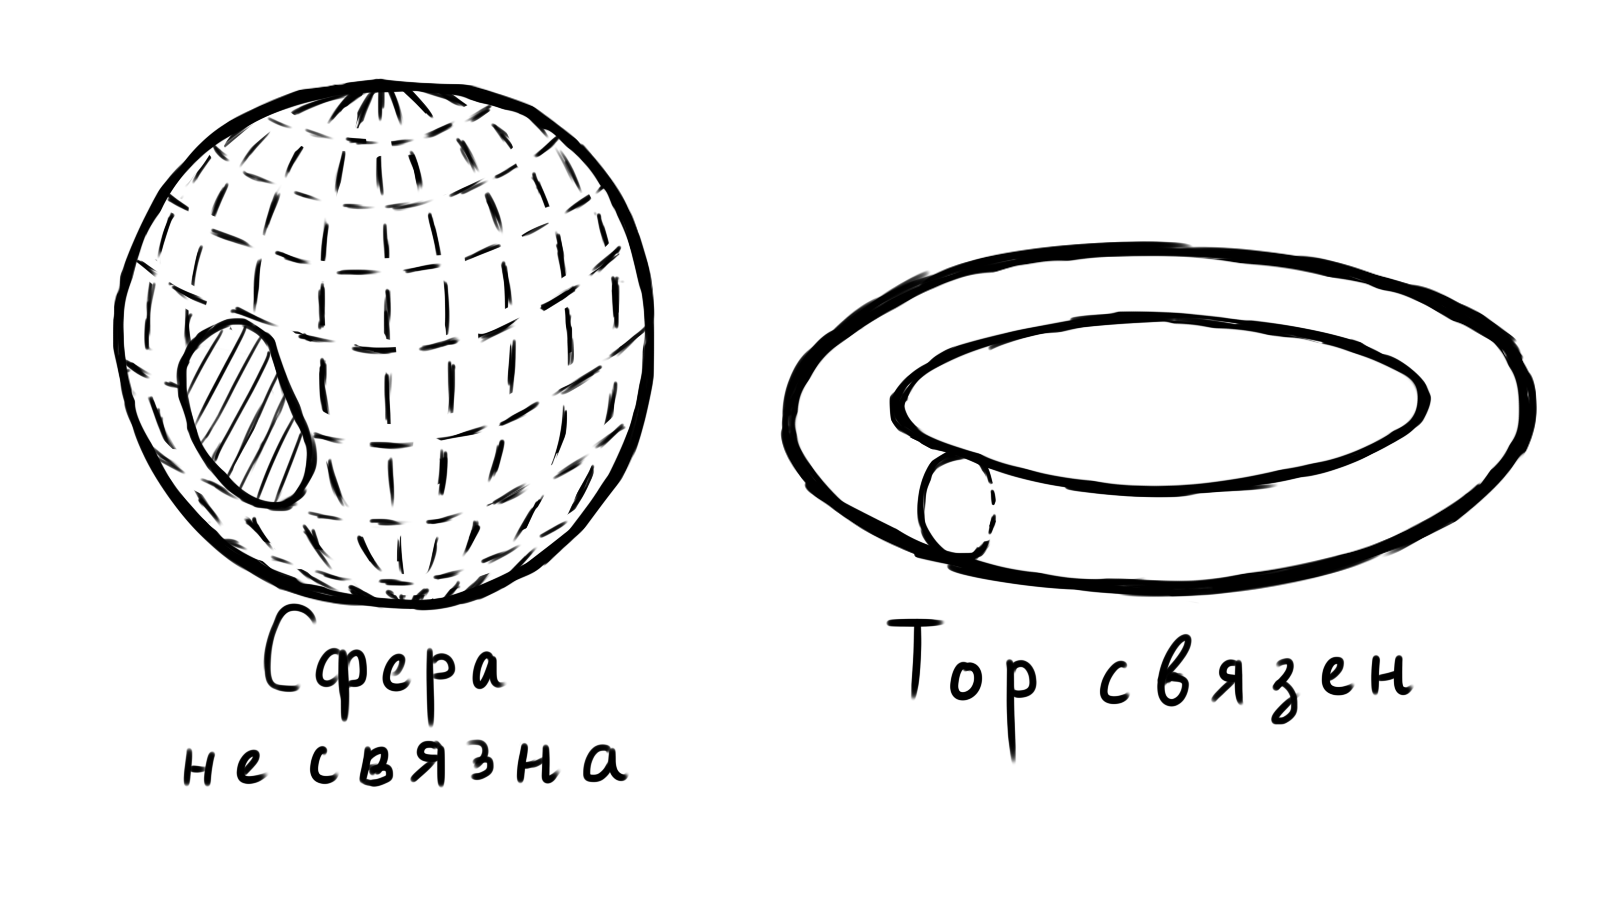
\includegraphics[width=0.5\textwidth]{sphere-torus}
\end{figure}

Тор можно неформально представлять на квадрате со следующими свойствами: при переходе кривой через верхнюю сторону она
продолжается из нижней стороны в той же точке по вертикали; аналогично при переходе через правую сторону. Это свойство
обозначают сонаправленными стрелками (стрелки на вертикальных сторонах и горизонтальных стороны следует обозначить
по-разному: если их обозначают одинаково, то это значит, что при переходе кривой она продолжится сразу со всех стороны;
если их обозначить несонаправленно, то продолжение кривой должно быть от точки с противоположного края стороны).

\begin{figure}[h]
	\centering 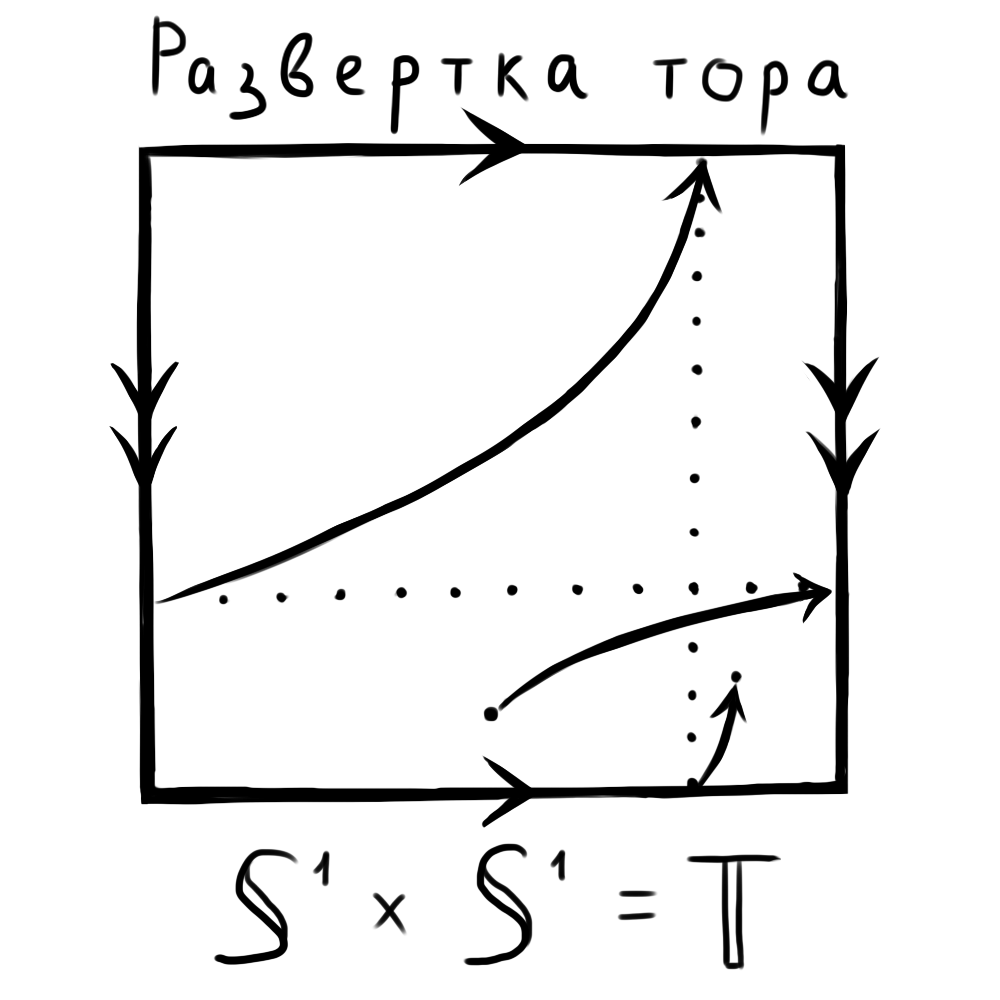
\includegraphics[width=0.3\textwidth]{dissection}
\end{figure}

Рассмотрим несколько примеров.

\begin{figure}[h]
	\centering 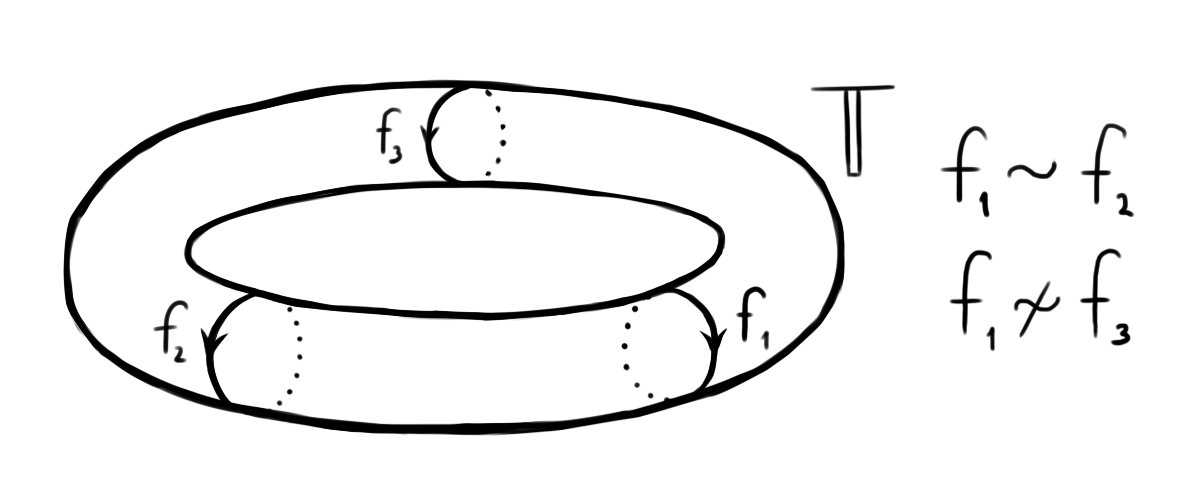
\includegraphics[width=0.5\textwidth]{torus-homotopy}
\end{figure}

Ясно, что $ f_1 $ и $ f_2 $ можно <<соединить>> однопараметрическим семейством отображений (в этом случае пишут
$ f_1 \sim f_2 $). Каждое из них есть <<такое же>> отображение, которое с ростом параметра $ t $ <<сдвинуто>> от
$ f_1 $ к $ f_2 $ на все большее расстояние и <<повернуто>> так, чтобы в итоге совместились начальные точки.
Однако отображения $ f_1 $, $ f_2 $ нельзя так же <<соединить>> с отображением $ f_3 $.

\begin{figure}[h]
	\centering 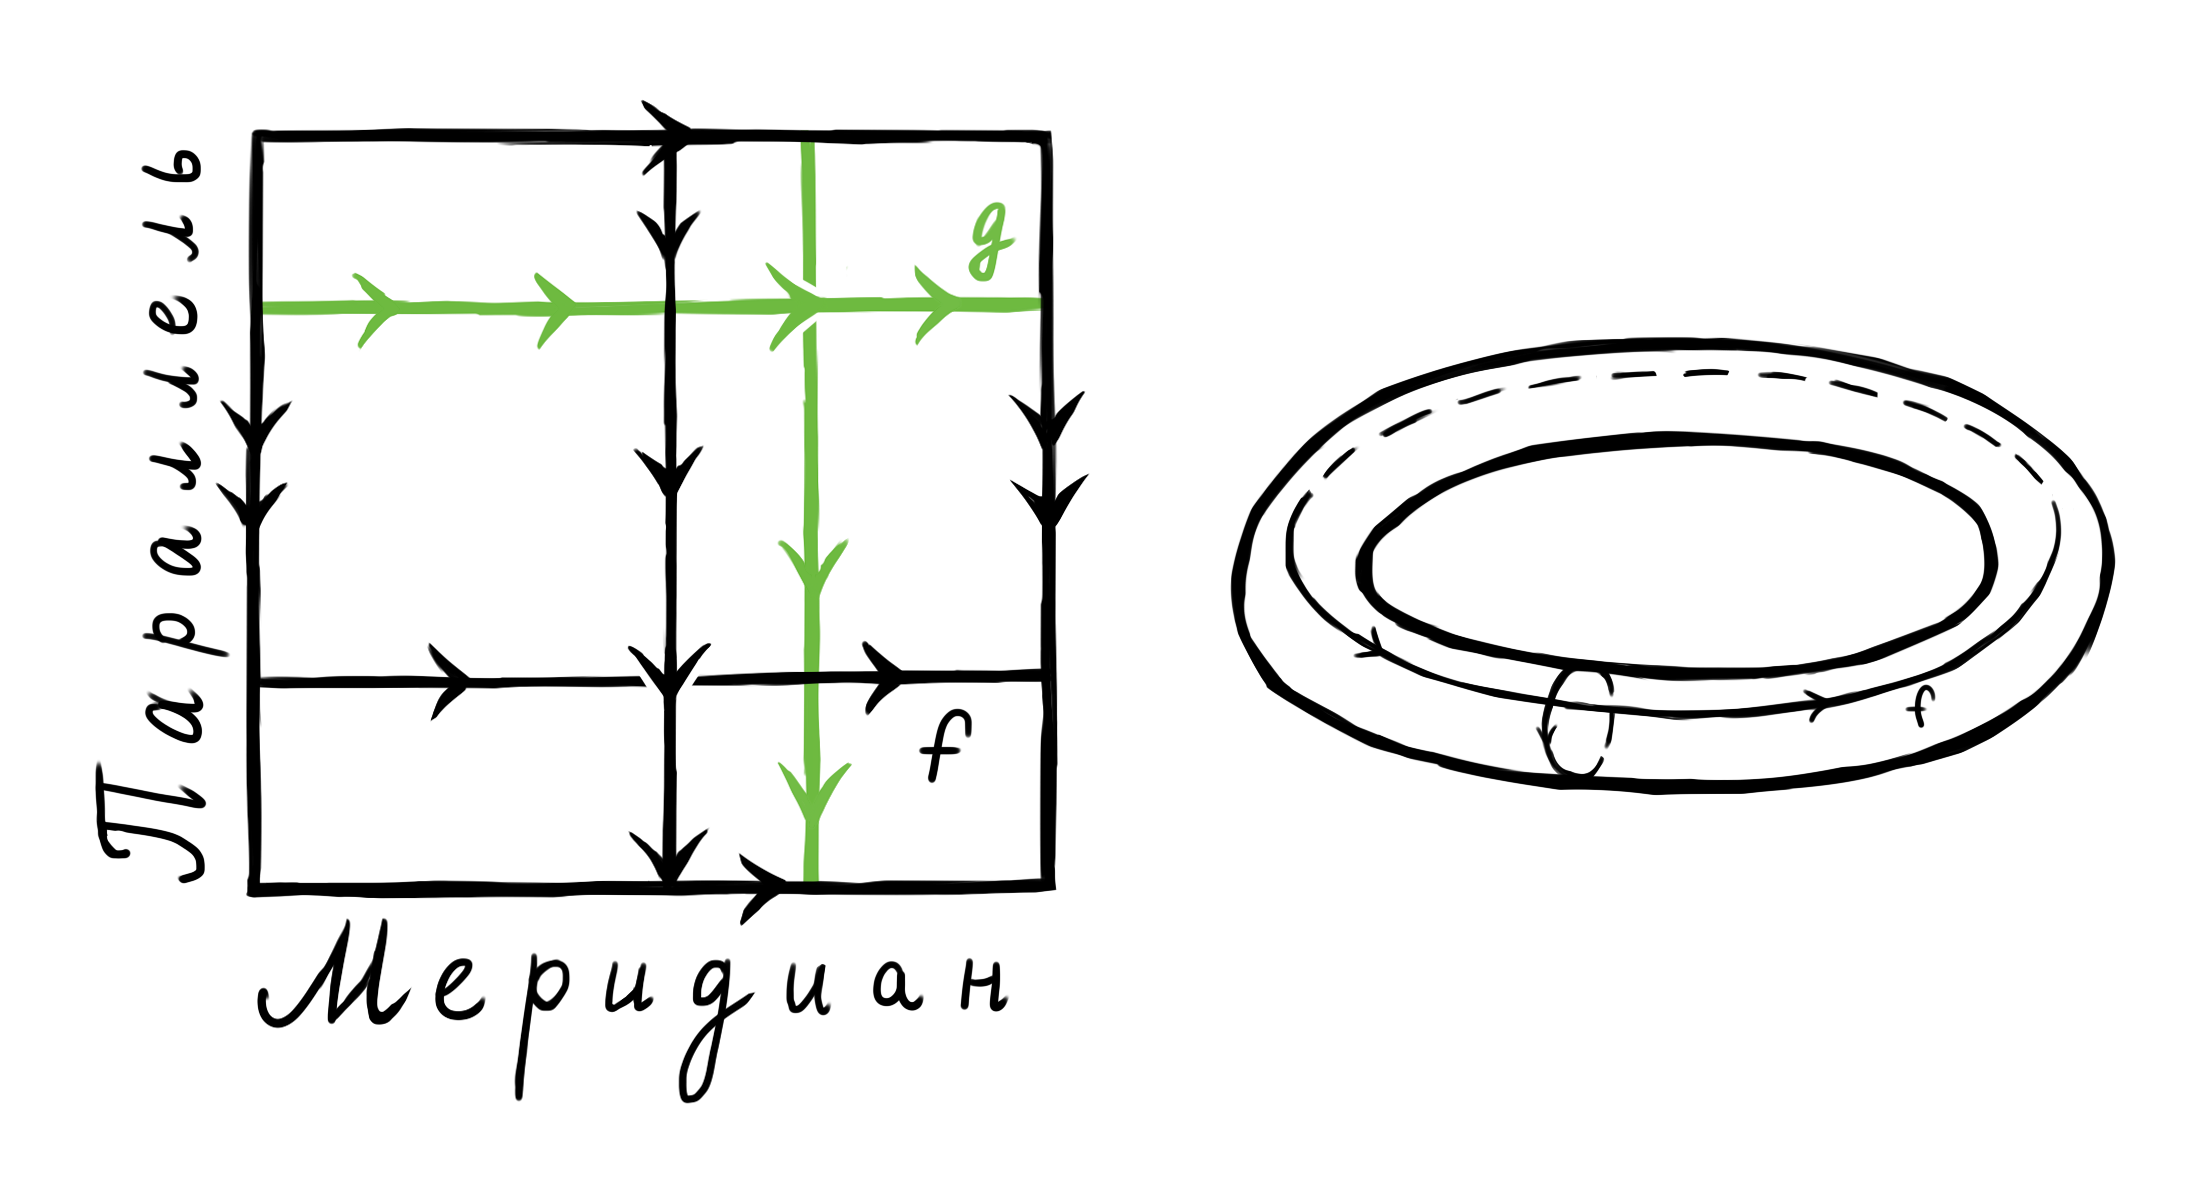
\includegraphics[width=0.5\textwidth]{parallel-meridian}
\end{figure}

Снова отображение окружности в тор. Одно отображение проходит сначала по меридиану тора, а потом по параллели; второе
--- наоборот. Их можно соединить непрерывным путем, и это показано с помощью изображения на развертке.

Такие <<соединяемые>> отображения называют гомотопными. Формулизуем это понятие.

\begin{definition}
	Пусть $ (T_1, \W_1), (T_2, \W_2) $ --- топологические пространства. Тогда:
	\begin{itemize}
		\item \emph{гомотопией между двумя непрерывными отображениями $ f_1, f_2 \colon T_1 \to T_2 $} называется такое
			непрерывное отображение $ F \colon T_1 \times [0; 1] \to T_2 $, что $ F(\cdot, 0) = f_1 $, а
		$ F(\cdot, 0) = f_2 $;
		\item если между двумя отображениями $ f_1, f_2 \colon T_1 \to T_2 $ существует гомотопия, то они
			называются \emph{гомотопными;} в этом случае пишут $ f_1 \sim f_2 $.
	\end{itemize}
\end{definition}

\begin{remark}
	Часто пишут $ f_t \colon T_1 \to T_2 $, где $ f_t(x) = F(t, x) $ для любого $ x \in T_1 $. Также можно задать и
	по-другому: пусть $ C(T_1, T_2) = \Set{ g \colon T_1 \to T_2 \mid g\text{ --- непрерывна} }$; теперь можно
	рассматривать некоторое отображение $ g \colon [0; 1] \to C(T_1, T_2) $.
\end{remark}

\begin{statement} \label{sta.4.1}
	Гомотопность является отношением эквивалентности.
\end{statement}

\begin{restatable}[из домашнего задания]{exercise}{ExcX}
	Композиция непрерывных отображений явдяется непрерывным отображением.
\end{restatable}

\begin{proof}[Доказательство утверждения \ref{sta.4.1}]
	Пусть $ (T_1, \W_1) $, $ (T_2, \W_2) $ --- топологические пространства.
	\begin{phased}
		\item[Рефлексивность.] Пусть $ f \colon T_1 \to T_2 $ --- непрерывное отображение. Определим отображение
			$ F \colon (x, t) \mapsto f(x) $ для любых $ x \in T_1 $ и $ t \in [0; 1] $. Тогда $ F = f \circ p_1 $,
			где $ p_1 \colon T_1 \times [0; 1] \to T_1 $ --- проекция на первую координату. Ясно, что $ p_1 $
			непрерывно, так как для любого открытого множества $ U \in \W_1 $ верно
			$ p_1^{-1}(U) = U \times [0; 1] \in B $, где $ B $ --- система окрестностей для декартова произведения.
			Таким образом, $ F $ непрерывна как композиция непрерывных отображений, $ f_0 = f = f_1 $, то есть это
			гомотопия.
		\item[Симметричность.] Пусть $ f_1, f_2 \colon T_1 \to T_2 $ --- непрерывные отображения и между ними есть
			гомотопия $ F \colon T_1 \times [0; 1] \to T_2 $, то есть $ F(\cdot, 0) = f_1 $,
			$ F(\cdot, 1) = f_2 $ и $ F $ непрерывно. Определим $ F' \colon T_1 \times [0; 1] \to T_2 $
			следующим образом: для $ x \in T_1 $ и $ t \in [0; 1] $ положим $ F'(x, t) = F(x, 1 - t) $.
			Тогда $ F'( \cdot, 0) = f_2 $, $ F'( \cdot, 1) = f_1 $. Докажем, что $ F' $ непрерывно.
			Рассмотрим отображения $ i_2 \colon t \mapsto 1 - t $, $ p_2 \colon T_1 \times [0; 1] \to [0; 1] $ ---
			проекция на вторую координату, затем $ i_1 = i_2 \circ p_2 $, $ p_1 \colon T_1 \times [0; 1] \to T_1 $ ---
			проекция на первую координату и, наконец, $ i = (p_1, i_1 )$. Тогда $ F' = F \circ i $: действительно,
			для любых $ x \in T_1 $ и $ t \in [0; 1] $ верно
				\[ F(i(x, t)) = F(p_1(x, t), i_1(x, t)) = F(x, (i_2(p_2(x, t))) =
				F(x, i_2(t)) = F(x, 1 - t) = F'(x, t). \]
			Таким образом, достаточно доказать непрерывность отображения $ i = (p_1, i_1) $. Так как проекция
			непрерывна, то достаточно доказать непрерывность отображения $ i_1 = i_2 \circ p_2 $. Так как проекция
			непрерывна, то достаточно доказать непрерывность отображения $ i_2 \colon t \mapsto 1 - t $. Его
			непрерывность очевидна.
		\item[Транзитивность.]
			\begin{lemma} \label{lem.4.1}
				Пусть $ (T_1, \W_1) $, $ (T_2, \W_2) $ --- топологические пространства, $ n \in \N $,
				$ T = \bigcup_{j = 1}^{n} A_j $, причем для любого $ j \in \Set{1, \ldots, n} $ множество $ A_j $
				замкнуто. Пусть $ f \colon T_1 \to T_2 $ --- некоторое отображение. Тогда если для любого
				$ j \in \Set{1, \ldots, n} $ отображение $ f_{A_j} $ непрерывно, то и отображение $ f $ также
				непрерывно.
			\end{lemma}
			Пусть $ f_1, f_2, f_3 \colon T_1 \to T_2 $ --- непрерывные отображения,
			$ F, G \colon T_1 \times [0; 1] \to T_2 $ --- гомотопии между $ f_1, f_2 $ и между $ f_2, f_3 $
			соответственно. Определим $ H \colon T_1 \times [0; 1] \to T_2 $ следующим образом: для любых
			$ x \in T_1 $ и $ t \in [0; 1] $ положим
				\[ H(x, t) = \begin{cases}
						F(x, 2 t), & \text{если } t \in \left[ 0; \frac{1}{2} \right]; \\
						G(x, 2 t - 1), & \text{если } t \in \left[\frac{1}{2}; 1 \right].
					\end{cases} \]
			Заметим, что элемент $ H \left( x, \frac{1}{2} \right) $ корректно определен и равен $ f_2(x) $ для любого
			$ x \in T_1 $. Ясно, что $ H(\cdot, 0) = f_1 $ и $ H(\cdot, 1) = f_3 $. Осталось доказать его
			непрерывность. По лемме достаточно доказать непрерывность отображения $ H $ на каждой половине отрезка
			$ [0; 1] $. Положим $ i_1 = (p_1, 2 p_2) $, где
			$ p_1 \colon T_1 \times \left[ 0; \frac{1}{2} \right] \to T_1 $ и
			$ p_2 \colon T_1 \times \left[ 0; \frac{1}{2} \right] \to \left[ 0; \frac{1}{2} \right] $ --- проекции на
			первую и вторую координату соответственно. Они непрерывны. Отображение $ 2 p_1 $ также, очевидно,
			непрерывно, так как это линейное преобразование отрезка. Значит, $ i_1 $ непрерывно. Но
			$ H_{\left[ 0; \frac{1}{2} \right]} = F \circ i_1 $, а значит, оно непрерывно.
			Аналогично доказывается непрерывность отображения $ H_{\left[ \frac{1}{2}; 1 \right]} $.
	\end{phased}
	Таким образом, гомотопность является отношением эквивалентности.
\end{proof}

\begin{proposition} \label{pro.4.1}
	Пусть $ (T_1, \W_1) $, $ (T_2, \W_2) $ --- топологические пространства, а $ f \colon T_1 \to T_2 $ --- некоторое
	отображение. Тогда отображение $ f $ непрерывно $\iaoi$ для любого замкнутого множества $ A \ssq T_1 $ множество
	$ f^{-1}(A) $ также замкнуто.
\end{proposition}

\begin{restatable}{exercise}{ExcXI}
	Пусть $ A \ssq T $, $ A_1 \ssq A $, причем $ A $ замкнуто в $ T $ и $ A_1 $ замкнуто в $ A $. Тогда множество
	$ A_1 $ замкнуто в $ T $.
\end{restatable}

\begin{restatable}{exercise}{ExcXII}
	Объединение конечного числа замкнутых множеств замкнуто.
\end{restatable}

\begin{proof}[Доказательство леммы \ref{lem.4.1}]
	Рассмотрим произвольное замкнутое множество $ A \ssq T_2 $. Тогда для любого $ j \in \Set{1, \ldots, n} $
	множество $ (f_{A_j})^{-1}(A) $ также замкнуто. Но тогда множество
		\[ f^{-1}(A) = f^{-1}(A) \cap \left( \bigcup_{j = 1}^n A_j \right) =
			\bigcup_{j = 1}^n \left( f^{-1}(A) \cap A_j \right) =
			\bigcup_{j = 1}^n (f_{A_j})^{-1}(A) \]
	тоже замкнуто как конечное объединение замкнутых множеств. Тогда в силу предложения отображение $ f $
	непрерывно.
\end{proof}

\begin{proof}[Доказательство предложения \ref{pro.4.1}] \leavevmode
	\begin{multiproof}
		\item[$\Then$] Все замкнутые множества --- это дополнения до всех открытых. Тогда для любого замкнутого
			множества $ A \ssq T_2 $ существует множество $ T_2 \wo A $, которое открыто. Следовательно, множество
			$ T_2 \wo f^{-1}(U) = f^{-1}(T_2 \wo A) $ открыто, то есть $ f^{-1}(A) $ замкнуто, что и требовалось.
		\item[$\If$] Все открытые множества --- это дополнения до всех замкнутых. Тогда для любого открытого
			множества $ U \in \W_2 $ существует множество $ T_2 \wo U $, которое замкнуто. Следовательно, множество
			$ T_2 \wo f^{-1}(U) = f^{-1}(T_2 \wo U) $ тоже замкнуто, то есть $ f^{-1}(U) $ открыто, что и требовалось.
	\end{multiproof}
\end{proof}

\begin{definition}
	Пусть $ X, Y $ --- топологические пространства. Обозначим через $ \pi(X, Y) $ множество всех классов гомотопности
	отображений из $ X $ в $ Y $.
\end{definition}

С помощью этого понятия можно, например, доказать негомеоморфность тора и сферы, что мы показывали раньше. Например,
$ \Abs{\pi(\S^1, \S^2)} = 1$, а $ \Abs{\pi(\S^1, \T)} = +\Inf$. Первое сразу понятно, так как все
отображения окружности в сферу гомеоморфны отображению окружности в заданную точку (например, в северный полюс) на
сфере. Второе мы докажем позже. Более того, мы увидим, что множество $\pi(\S^1, \T)$ в некотором смысле
обладает групповой структурой и называется фундаментальной группой пространства $ \T $.

\subsection{Фундаментальная группа топологического пространства}

\begin{definition}
	Пусть $X$ и $ Y $ --- топологические пространства, $ A \ssq X $, $ B \ssq Y $ --- некоторые их непустые
	подмножества. Тогда отображение $ f \colon X \to Y $ называется отображением $ f \colon (X, A) \to (Y, B) $
	пар топологических пространств, если оно непрерывно и $ f(A) \ssq B $.
\end{definition}

\begin{definition}
	Пусть $X$ и $ Y $ --- топологические пространства, $ A \ssq X $, $ B \ssq Y $ --- некоторые их непустые
	подмножества, $ f_1, f_2 \colon (X, A) \to (Y, B) $ --- отображения пар. Тогда они называются \emph{гомотопными},
	если между ними сущесвует такая гомотопия $ F \colon X \times [0; 1] \to Y $, что $ F(A \times [0; 1]) \ssq B $
	(или, что то же самое, для любого $ t \in [0; 1] $ верно $ F(A, t) \ssq B $).
\end{definition}

\begin{definition}
	Пусть $X$ и $ Y $ --- топологические пространства, $ A \ssq X $, $ B \ssq Y $ --- некоторые их непустые
	подмножества. Тогда через $ \pi((X, A), (Y, B))$ обозначается множество классов гомотопности отображений пар
	топологических пространств.
\end{definition}

\begin{definition}
	\emph{Фунадментальной группой} топологического пространства $ X $ с выделенной точкой $ x_0 \in X $ называется
	множество $ \pi_1(X, x_0) = \pi(([0; 1], \Set{0, 1}), (X, \Set{x_0})) $.
\end{definition}

\begin{remark}
	Отображения пар $ \colon ([0; 1], \Set{0, 1}) \to (X, \Set{x_0}) $ называют петлями. Мы помним, что отображения из
	отрезка $ [0; 1] $ в топологическое пространство называются путями. Здесь также пути, однако точки $ 0 $ и $ 1 $
	переходят в заданную точку $ x_0 $ согласно определению отображения пар. Таким образом, получается замкнутая
	кривая.
\end{remark}

\begin{restatable}{theorem}{FactorSetIsGroup}
	Множество $ \pi_1(X, x_0) $ классов гомотопности петель является группой относительно следующей операции:
	пусть $ a $, $ b $ --- петли, тогда положим $ [b][a] = [ba] $, где
		\[ (ba)(t) = \begin{cases}
				a(2 t), & \text{если } t \in \left[ 0; \frac{1}{2} \right]; \\
				b(2 t - 1), & \text{если } t \in \left[ \frac{1}{2}; 1 \right].
			\end{cases}
		\]
\end{restatable}

\begin{remark}
	В точке $ t = \frac{1}{2} $ отображение $ ba $ корректно определено и равно $ x_0 $.
\end{remark}

\begin{remark}
	Для доказательства теоремы необходимо доказать корректность (почему произведение классов эквивалентности
	не зависят от выбора петель $ a $ и $ b $ внутри них), ассоциативность, существование нейтрального и
	обратного элементов.
\end{remark}

\end{document}